\documentclass[final,3p,times,twocolumn]{elsarticle}

%% Use the option review to obtain double line spacing
%% \documentclass[preprint,review,12pt]{elsarticle}

%% Use the options 1p,twocolumn; 3p; 3p,twocolumn; 5p; or 5p,twocolumn
%% for a journal layout:
%% \documentclass[final,1p,times]{elsarticle}
%% \documentclass[final,1p,times,twocolumn]{elsarticle}
%% \documentclass[final,3p,times]{elsarticle}
%% \documentclass[final,3p,times,twocolumn]{elsarticle}
%% \documentclass[final,5p,times]{elsarticle}
%% \documentclass[final,5p,times,twocolumn]{elsarticle}

%% if you use PostScript figures in your article
%% use the graphics package for simple commands
%% \usepackage{graphics}
%% or use the graphicx package for more complicated commands
%% \usepackage{graphicx}
%% or use the epsfig package if you prefer to use the old commands
%% \usepackage{epsfig}

%% The amssymb package provides various useful mathematical symbols
\usepackage{amssymb}
%% The amsthm package provides extended theorem environments
%% \usepackage{amsthm}
%% The bm package lets you access bold symbols in math mode using the \boldsymbol command (useful to get bold greek letters).
\usepackage{bm}
%% The bbm package is contains the indicator function symbol \mathbbm{1}
\usepackage{bbm}
%% The amsmath package contains the split environment, letting you split equations into multiple lines.
%% See "https://www.sharelatex.com/learn/Aligning_equations_with_amsmath " for an explanation.
\usepackage{amsmath}
%% The lineno packages adds line numbers. Start line numbering with
%% \begin{linenumbers}, end it with \end{linenumbers}. Or switch it on
%% for the whole article with \linenumbers after \end{frontmatter}.
%% \usepackage{lineno}
%% The algorithm defines the algorithm floating environment and the algpseudocode package is useful for constructing Pseudo code.
\usepackage{algorithm}
\usepackage{algpseudocode}
%% Declaring \argmin and \argmax operators:
\DeclareMathOperator*{\argmin}{arg\,min}
\DeclareMathOperator*{\argmax}{arg\,max}
%% natbib.sty is loaded by default. However, natbib options can be
%% provided with \biboptions{...} command. Following options are
%% valid:

%%   round  -  round parentheses are used (default)
%%   square -  square brackets are used   [option]
%%   curly  -  curly braces are used      {option}
%%   angle  -  angle brackets are used    <option>
%%   semicolon  -  multiple citations separated by semi-colon
%%   colon  - same as semicolon, an earlier confusion
%%   comma  -  separated by comma
%%   numbers-  selects numerical citations
%%   super  -  numerical citations as superscripts
%%   sort   -  sorts multiple citations according to order in ref. list
%%   sort&compress   -  like sort, but also compresses numerical citations
%%   compress - compresses without sorting
%%
%% \biboptions{comma,round}

% \biboptions{}


\journal{MPhil in Scientific Computing}

\begin{document}

\begin{frontmatter}

%% Title, authors and addresses

%% use the tnoteref command within \title for footnotes;
%% use the tnotetext command for the associated footnote;
%% use the fnref command within \author or \address for footnotes;
%% use the fntext command for the associated footnote;
%% use the corref command within \author for corresponding author footnotes;
%% use the cortext command for the associated footnote;
%% use the ead command for the email address,
%% and the form \ead[url] for the home page:
%%
%% \title{Title\tnoteref{label1}}
%% \tnotetext[label1]{}
%% \author{Name\corref{cor1}\fnref{label2}}
%% \ead{email address}
%% \ead[url]{home page}
%% \fntext[label2]{}
%% \cortext[cor1]{}
%% \address{Address\fnref{label3}}
%% \fntext[label3]{}

\title{Mini Project: Implementation and comparison of the Gaussian Mixture model, the K-means algorithm and the Dirichlet Process}

%% use optional labels to link authors explicitly to addresses:
%% \author[label1,label2]{<author name>}
%% \address[label1]{<address>}
%% \address[label2]{<address>}

\author{Brian Azizi}

\address{Cavendish Laboratory, Department of Physics, J J Thomson
  Avenue, Cambridge. CB3 0HE}

\begin{abstract}
Abstract of the mini project. As part of the written assignment for the MPhil in Scientific Computing, I have implemented three clustering algorithms in the C++ programming language, the k-means algorithm, the Gaussian mixture model and the Dirichlet Process. Subsequently, the algorithms will be compared and texted on a number of data sets.
\end{abstract}

\end{frontmatter}

%%
%% Start line numbering here if you want
%%
% \linenumbers

%% main text
\section{Introduction}
\label{sect:Intro}
Clustering is part of unseupervised machine learning. Given a set of unlabeled data, the aim is to find clusters of data points, such that data points within a cluster are similar to each other and different to data points not in that cluster.
A word on notation. Each training example is a vector in $D$-dimensional space, $\mathbb{R}^D$, and each component of the vector is a feature. A particular training example is denoted $\mathbf{x}^{(i)} \in \mathbb{R}^D$. The training examples are indexed by $i$ and we have $N$ training examples, thus $i \in \{1,2,\dots ,N\}$. The features are indexed with the letter $j$, $j \in \{1,2,\dots,D\}$. The letter $K$ is used to denote the number of clusters.

We will focus on three different clustering algorithms: K-means \cite{lloyd1982}, Gaussian mixtures and the Dirichlet Process. \emph{K-means} is arguably the least complex out of those three models. The number of clusters, $K$, is a hyper-parameter of the model that needs to be set by the user, thus making it a \emph{parametric model}. K-means assigns each data point to one of the clusters and gives us the location of each cluster. It performs \emph{hard clustering}, meaning each data point is assigned to a cluster without any measure of confidence. Contrast this with the \emph{Gaussian Mixture model} which supplies us with the probability of each data point belonging to each of the individual clusters. This \emph{soft clustering} is desirable, as it allows for \emph{anomaly detection}. However, the number of clusters is still set manually and different values for $K$ can lead to very different models. Our third model, the \emph{Dirichlet process}, deals with this problem by infering from the data what the optimal number of clusters is. It is a \emph{non-parametric} model.
 
\section{K-Means Clustering}
In K-Means, we explicitly choose the number of clusters, $K$, into which we would like to partition our data set. Intuitively, data points in the same cluster should have small distance between them compared to the distance of data points in different clusters. To this end, the K-Means method finds $K$ \emph{cluster centroids}, one for each cluster, and assigns a single label to every data point corresponding to the closest centroid. 

We denote the $k$th centroid by $\boldsymbol{\mu}_k \in \mathbb{R}^D$, $k \in \{1, \dots, K\}$ and the label, or \emph{index}, of the $i$th example by $c^{(i)} \in \{1, \dots, K\}$. We can state the optimization objective of the K-Means method:
\begin{equation}
\begin{split}
\min_{c^{(1)},\dots,c^{(N)},\boldsymbol{\mu}_1,\dots,\boldsymbol{\mu}_K} &J(c^{(1)},\dots,c^{(N)},\boldsymbol{\mu}_1,\dots,\boldsymbol{\mu}_K) \\
&= \frac{1}{N}\sum_{i=1}^N ||\boldsymbol{x}^{(i)} - \boldsymbol{\mu}_{c^{(i)}}||^2
\end{split}
\label{eqn:kmeansCost}
\end{equation}
The objective function $J$ is sometimes referred to as the \emph{distortion measure} or the \emph{cost function}. We can use an iterative procedure to minimize $J$. We start out by choosing some initial values for the cluster centroids $\boldsymbol{\mu}_k$. In each iteration step, we first assign an index to each example that corresponds to the closest centroid. Subsequently, we update each centroid $\boldsymbol{\mu}_k$ by setting them equal to the mean of all examples that are currently assigned to their respective clusters $k$. We repeat these two steps until no more changes occur and we converge.

\begin{algorithm}
\caption{K-Means algorithm}
\label{alg:kmeans}
\begin{algorithmic}[1]
\Procedure{K-Means}{$X,K$}
\State{Randomly initialize $K$ cluster centroids in $\mathbb{R}^D$}
\Repeat
\For{$i = 1:N$}
\State{$c^{(i)} = \argmin_k ||\boldsymbol{x}_i - \boldsymbol{k}_k||$}
\EndFor
\For{$k = 1:K$}
\State{$N_k = \sum_{i=1}^N \mathbbm{1}\{c^{(i)} = k \}$}
\State{$\boldsymbol{\mu}_k = \sum_{i:c^{(i)}=k} \boldsymbol{x}^{(i)} / N_k$}
\EndFor
\Until{Convergence}\Comment{No more changes}
\EndProcedure \\
\Return{$c^{(1)}, \dots, c^{(N)}, \boldsymbol{\mu}_1, \dots, \boldsymbol{\mu}_K $}
\end{algorithmic}
\end{algorithm}

In figure \ref{fig:kmeans1} we have set $K = 3$.
\begin{figure}
\centering
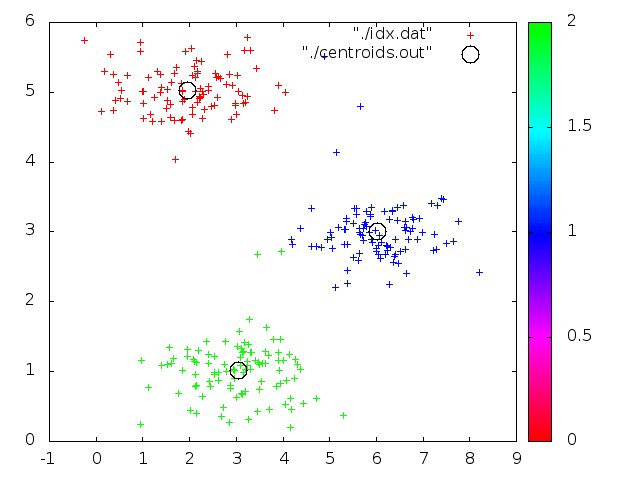
\includegraphics[width=3in]{kmeans1.png}
\caption{Result of running the K-Means algorithm on the toyclusters dataset with $K=3$}
\label{fig:kmeans1}
\end{figure}

\section{The Gaussian Mixture Model}
The Gaussian Mixture Model (GMM) is perhaps the most widely used latent variable model for clustering. A common method for density estimation is to assume the data comes from a Gaussian distribution. One then proceeds to form the likelihood model and maximise it in order to get an estimate for the parameters of the model. In the GMM, we take this one step further and assume that the comes from one of $K$ possible Gaussians. For each sample $\boldsymbol x$, there is a corresponding \emph{latent variable} $\boldsymbol z$ that indicates which one of the Gaussians was responsible for $\boldsymbol x$.



\section*{Acknowledgements}
Here I acknowledge the assistance of my supervisor, my industrial sponsor,
and the effects of caffine on my ability to produce this report on time.

%% The Appendices part is started with the command \appendix;
%% appendix sections are then done as normal sections
\appendix

\section{On the Derivation of the Quadratic Formula}
\label{app:quad}
The derivation of the quadratic formula is something that would not
fit well within a paper as it would interrupt the flow of the argument
therein. However, for those students who need a refresher on how the
quadratic formula is derived, we give full details here:\par
Assume that we have
\begin{equation}
p(x) = ax^2 + bx + c
\end{equation}
and so on. The actual algebra is left as an exercise for the reader.

%% References
%%
%% Following citation commands can be used in the body text:
%% Usage of \cite is as follows:
%%   \cite{key}         ==>>  [#]
%%   \cite[chap. 2]{key} ==>> [#, chap. 2]
%%

%% References with bibTeX database:
\section*{Bibliography}
\bibliographystyle{elsarticle-num}
\bibliography{references.bib}

%% Authors are advised to submit their bibtex database files. They are
%% requested to list a bibtex style file in the manuscript if they do
%% not want to use elsarticle-num.bst.

%% References without bibTeX database:

% \begin{thebibliography}{00}

%% \bibitem must have the following form:
%%   \bibitem{key}...
%%

% \bibitem{}

% \end{thebibliography}


\end{document}

%%
%% End of file `mini.tex'.